\chapter{Visão Geral dos Subsistemas}

A integração do sistema configura-se como fator decisivo para o cumprimento dos objetivos definidos.
Sendo assim, elaborou-se o esquemático, conforme figura \ref{fig:visao_geral}, com a finalidade de fornecer uma visão geral a
respeito dos principais aspectos de integração dos subsistemas.

\begin{figure}[!htbp]
\begin{center}
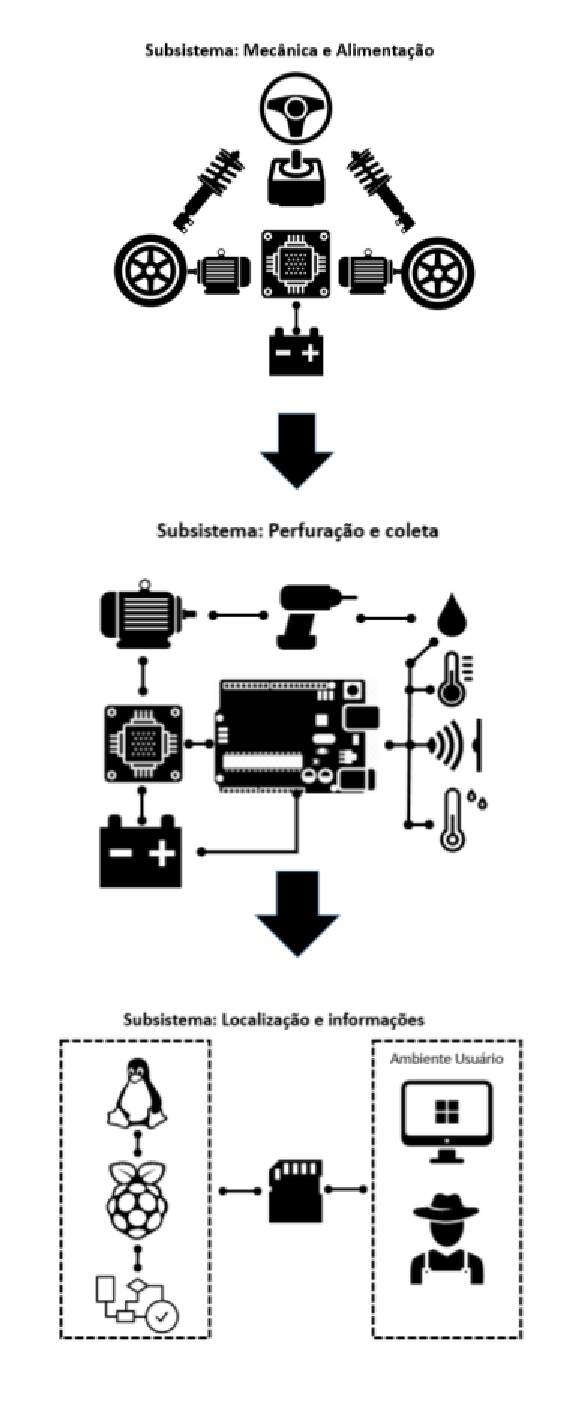
\includegraphics[width=.6\textwidth]{figuras/all_systems.eps}
\caption{\label{fig:visao_geral}Visão geral do sistema.}
\end{center}
\end{figure}

% Talvez quebrar a imagem em 3

O subsistema de Mecânica e alimentação é composto por tração, direção, estrutura e alimentação. O motor
responsável pela tração das rodas será controlado por um driver, que por sua vez receberá sinais lógicos da placa Arduino
para a determinação do sentido de rotação e velocidade angular. Este driver será alimentado pela bateria do sistema conforme
figura \ref{fig:visao_geral} (diagrama unifilar). Em conjunto aos elementos de tração, a direção também será integrada de forma
a compor o chassi do veículo. Por fim, os elementos mencionados serão integrados à estrutura, mais especificamente à carroceria.

Vale ressaltar que o projeto da carroceria deve considerar em seu espaço interno todos os componentes eletrônicos, de
alimentação e de perfuração.

Sendo assim, percebe-se que o subsistema de perfuração e coleta apresenta alto grau de integração com os demais subsistemas.
Tendo como núcleo central a placa Arduino, esse subsistema tem como objetivo realizar a coleta dos dados provenientes dos
sensores. Seu ponto crítico de integração consiste em projeto e alocação do sistema de perfuração, responsável por introduzir
o sensor de umidade de solo no ponto desejado sem causar danos ao mesmo. Todos os componentes eletromecânicos do subsistema,
também serão alimentados pela bateria.

%\vfill
%\pagebreak

Os dados adquiridos pelos sensores e lidos pela placa Arduino, serão enviados para a unidade de processamento, composta por
uma placa Raspberry Pi, um sistema operacional Linux embarcado, o qual executará o algoritmo de localização do sistema. Este
algoritmo irá tomar decisões a respeito de onde o veículo estará no ambiente, e as enviará para o conjunto Arduino/Driver, por meio de uma UART, visando o controle de
direção. Além disso, esse algoritmo será responsável por armazenar os dados referentes à coleta em seus respectivos
pontos. Este armazenamento será implementado na Raspberry Pi, que estará disponível para posterior visualização por
parte do usuário final.

\chapter{Plano de Integração e Testes}

Dado a execução das atividades planejadas ate o úlmtimo plano de controle e a atual situação dos subsistemas, abaixo estão listados o planejamento da integração e teste dos componentes de cada subsistema e a integração e teste de todos os subsistemas para a construção do produto final.

\section{Subsistema: Mecânica e Alimentação}

\section{Subsistema: Perfuração e Coleta}

\section{Subsistema: Localização e Informações}

Em relação as integrações neste subsistema, a parte do sistema para o usuário não possui muita dependência com as outras partes do projeto. A depedência que possui é a parte de envio e recebimento dos dados através da rede usando os protocolos tcp e ftp que já foram explicados anteriormente neste trabalho.

Assim, para a integração, depende apenas do servidor que está rodando na raspberry enviar e receber corretamente os arquivos com os dados. Desse modo a integração dessa parte já foi feita dentro deste subsistema, onde posteriormente será realizado os testes do envio e recebimento dos arquivos via ftp e envio do comando via tcp que vai dar o start no carro. 

Os sensores já conseguem coletar os dados, e mandar para a raspberry, então será realizado os testes primeiramente se o sistema consegue receber os arquivos com os dados coletados dos sensores de umidade do solo, umidade do ar e temperatura do ar. Depois testar se o servidor na raspberry consegue receber os arquivo com os dados de .... e o comando que inicia o carro.

Para o sistema de localização ...

\section{Integração Geral dos Subsistemas}


